\documentclass[spanish,letterpaper,oneside]{article}

% Datos del documento
\def\documenttitle {Diagnóstico de enseñanza, aprendizaje, paradigmas y matemáticas}
\def\documentsubtitle {Fundamentos para la enseñanza y el aprendizaje I}
\def\documentsubject {Actividad 1 · Reflexión inicial}
\def\documentauthor {Mtro. Martín Jonathan de la Cruz Muñoz}
\def\coursename {Fundamentos para la enseñanza y el aprendizaje I}
\def\coursecode {MAEM}

% Identidad institucional
\def\universityname {Instituto de Investigación, Innovación y Estudios de Posgrado para la Educación del Estado de Nuevo León}
\def\universityfaculty {Maestría en Aprendizaje y Enseñanza de las Matemáticas}
\def\universitydepartment {Fundamentos para la enseñanza y el aprendizaje I}
\def\universitydepartmentimage {img/iiiepe/marca-iiiepe.png}
\def\universitydepartmentimagecfg {height=1.75cm}
\def\universitylocation {Monterrey, Nuevo León}
\def\studentfullname {Mtro. Martín Jonathan de la Cruz Muñoz}
\def\studentid {00874}
\def\studentemail {martin.delacruz@campus.iiiepe.edu.mx}
\def\programperiod {1er tetramestre, marzo--julio de 2026}
\def\programmodality {Modalidad presencial}
\def\programshort {MAEM}

\def\authortable {
  \begin{tabular}{ll}
    \textbf{Alumno:} & \studentfullname \\
    Matrícula: & \studentid \\
    Correo institucional: & \studentemail \\
    Unidad: & \coursename \\
    Programa: & \programshort \\
    Periodo: & \programperiod \\
    & \\
    \multicolumn{2}{l}{Fecha de realización: 13 de octubre de 2026} \\
    \multicolumn{2}{l}{\universitylocation}
  \end{tabular}
}

\input{template}

\usepackage{helvet}
\renewcommand{\familydefault}{\sfdefault}
\usepackage{array}
\usepackage{longtable}
\usepackage{pdflscape}
\usepackage{tikz}
\usepackage[most]{tcolorbox}
\usetikzlibrary{arrows.meta,positioning,calc,fit,backgrounds}

\definecolor{iiiepeNavy}{HTML}{163B5C}
\definecolor{iiiepeBlue}{HTML}{1F6F9F}
\definecolor{iiiepeAqua}{HTML}{20B7A8}
\definecolor{iiiepeOrange}{HTML}{F28C28}
\definecolor{iiiepePaper}{HTML}{F6F8F7}
\definecolor{iiiepeInk}{HTML}{1E2A32}
\def\portraittitlecolor {iiiepeNavy}
\setcitestyle{authoryear,open={(},close={)}}

\newcommand{\insertcoverwatermark}{%
  \AddToShipoutPictureBG*{%
    \begin{tikzpicture}[remember picture,overlay]
      \node[opacity=.09,inner sep=0pt] at (current page.center)
      {\includegraphics[width=.58\paperwidth]{img/iiiepe/logo-puntos.png}};
    \end{tikzpicture}%
  }%
}

\newtcolorbox{reportelecturabox}[1][]{%
  enhanced,breakable,
  colback=iiiepePaper,colframe=iiiepeNavy,
  boxrule=1pt,leftrule=4pt,arc=2pt,
  left=8pt,right=8pt,top=6pt,bottom=6pt,
  before skip=6pt,after skip=10pt,
  fonttitle=\bfseries\color{white},coltitle=white,
  colbacktitle=iiiepeNavy,
  attach boxed title to top left={xshift=8pt,yshift=-2pt},
  boxed title style={colback=iiiepeNavy,colframe=iiiepeNavy,arc=1pt},
  title={Reporte de lectura},#1}

\newtcolorbox{fichalecturabox}[1][]{%
  enhanced,breakable,
  colback=iiiepeAqua!7,colframe=iiiepeAqua!70!iiiepeNavy,
  boxrule=.6pt,arc=1pt,
  left=7pt,right=7pt,top=4pt,bottom=4pt,
  fontupper=\small,before upper={\setstretch{1.0}},
  fonttitle=\bfseries\color{iiiepeNavy},coltitle=iiiepeNavy,
  colbacktitle=iiiepeAqua!7,
  title={Ficha de la lectura},#1}



\usepackage{tabularx,colortbl,pgfplots,enumitem,needspace}\pgfplotsset{compat=1.18}\definecolor{iiiepePale}{HTML}{EEF5F8}
\setlength{\parskip}{5pt}\setlength{\parindent}{0pt}
\begin{document}\insertcoverwatermark\templatePortrait\templatePagecfg\templateFinalcfg\fancyfoot{}\fancyfoot[L]{\scriptsize IIIEPE · MAEM}\fancyfoot[C]{\scriptsize\thepage}\fancyfoot[R]{\scriptsize Actividad 1}\setstretch{1.3}\raggedbottom
\section{Una concepción docente en revisión}
Mi experiencia en CONALEP y CECyTE, en mantenimiento y mecatrónica, y en licenciaturas de Ingeniería Mecánica, de Sistemas e Industrial, me ha llevado a organizar la enseñanza desde la administración del conocimiento y del trabajo. La maestría me permite revisar ese punto de partida: la claridad técnica debe acompañarse de atención a la persona, a sus contextos y a la construcción de significado. Este diagnóstico expresa mi concepción actual, sin presentarla como una medición de resultados de aula.

\begin{center}
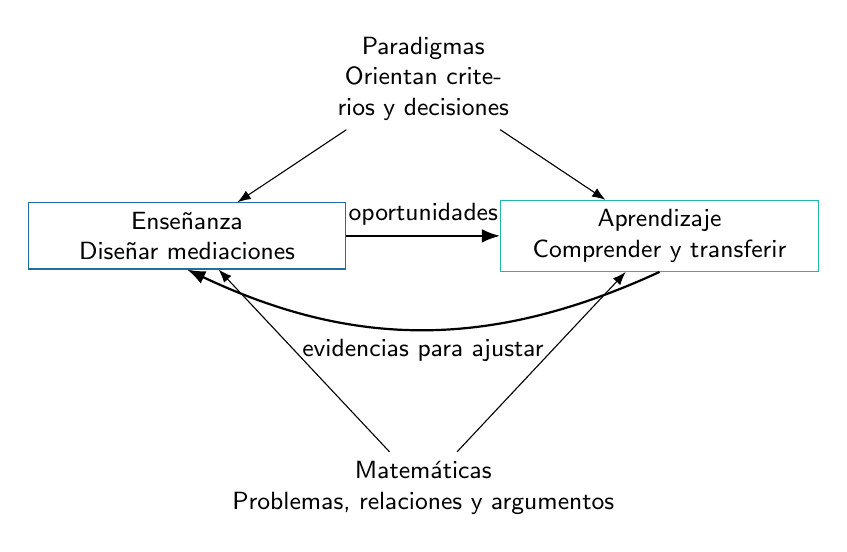
\begin{tikzpicture}[font=\small,>=Latex]
\node[draw=iiiepeBlue,align=center,text width=3.8cm] (e) at (0,0){Enseñanza\\Diseñar mediaciones};\node[draw=iiiepeAqua,align=center,text width=3.8cm] (a) at (6,0){Aprendizaje\\Comprender y transferir};
\node[align=center,text width=4cm] (p) at (3,2){Paradigmas\\Orientan criterios y decisiones};\node[align=center,text width=5cm] (m) at (3,-3.2){Matemáticas\\Problemas, relaciones y argumentos};\draw[->,thick] (e)--node[above]{oportunidades}(a);\draw[->,thick] (a.south) to[bend left=25] node[below]{evidencias para ajustar}(e.south);\draw[->] (p)--(e);\draw[->] (p)--(a);\draw[->] (m)--(e);\draw[->] (m)--(a);\end{tikzpicture}
\end{center}
\section{Enseñanza}
Entiendo la enseñanza como la organización intencional de condiciones, tareas y mediaciones para que otra persona comprenda, actúe y argumente con autonomía creciente. Explicar un procedimiento es una parte del proceso; también lo son escuchar una interpretación, reconocer un obstáculo y ofrecer una representación accesible. En una clase de mantenimiento, enseñar a calcular una tolerancia implica explicar su significado, justificar el procedimiento y valorar cómo se verifica, no solo mostrar una secuencia para copiar.
Mi cambio de perspectiva consiste en conservar objetivos y criterios claros, incorporando más diálogo sobre las razones del estudiante. La eficiencia del trabajo docente debe estar al servicio de la comprensión y no convertirse en el único criterio de valoración.
\section{Aprendizaje}
El aprendizaje es una transformación del conocimiento y de las posibilidades de actuar que permite comprender, relacionar y utilizar lo aprendido. Una respuesta correcta puede proceder de imitación; por eso buscaría explicaciones, transferencia y revisión de errores. En mecatrónica, ejecutar un programa no demuestra por sí mismo que se comprendan sus variables; explicar por qué una modificación cambia el movimiento ofrece otra evidencia.
Aprender también implica reconocer lo que aún no se domina y pedir apoyo. Desde una enseñanza humanista, esa necesidad no disminuye la dignidad ni el potencial de la persona. La evaluación debe orientar el siguiente paso y permitir utilizar la retroalimentación.
\section{Paradigmas}
Un paradigma es un marco de supuestos que orienta qué se considera conocimiento, cómo se aprende y qué se valora como evidencia. Una mirada centrada en transmisión y control puede privilegiar repetición y uniformidad; una mirada constructiva y sociocultural incorpora saberes previos, interacción y contexto. La perspectiva humanista agrega atención a la persona, su agencia y sus condiciones de desarrollo. Estos enfoques no se sustituyen con una etiqueta: se reconocen en las decisiones de clase.
Identifico en mi punto de partida una organización industrial del conocimiento. Su fortaleza es la trazabilidad de objetivos y procedimientos; su límite aparece si trato a todos los estudiantes como si tuvieran el mismo punto de partida. Mi revisión busca mantener el rigor e introducir apoyos, participación y criterios de comprensión.
\section{Matemáticas}
Concibo las matemáticas como una actividad de construcción y estudio de relaciones, estructuras y patrones mediante representaciones y argumentos. Su utilidad en ingeniería es evidente, pero su valor educativo también incluye razonar, justificar y examinar supuestos. Una fórmula es una relación con condiciones de validez, no una instrucción que pueda aplicarse a cualquier situación.
Por ejemplo, $d=vt$ requiere velocidad constante y una referencia definida; $d=vt+d_0$ incorpora una posición inicial. Distinguirlos conecta modelación con comprensión conceptual. Enseñaría a preguntar qué representa cada variable, qué unidades conserva y qué información permite aceptar o rechazar el modelo.
\section{Relación entre los cuatro conceptos}
La enseñanza organiza oportunidades; el aprendizaje se evidencia en cambios de comprensión; los paradigmas orientan decisiones; las matemáticas aportan un campo de problemas y argumentos. Mi propósito es que la disciplina del trabajo técnico conviva con una relación pedagógica que reconozca diferencias y permita revisar. La pregunta que llevaré a la maestría es cómo diseñar esa convivencia sin reducir exigencia ni participación.

\section{Un criterio que conecta las cuatro concepciones}
Una situación de mantenimiento puede formularse como comparación entre dos costos: $C_A(h)=250+80h$ y $C_B(h)=100+110h$. Enseñar supone preparar representaciones y preguntas; aprender se evidencia cuando el estudiante explica el significado de la cuota fija, encuentra $h=5$ y justifica qué alternativa conviene antes y después de ese punto. El paradigma aparece en la decisión de pedir solo el resultado o permitir contrastar estrategias y revisar una interpretación.
Las matemáticas aportan una estructura argumentativa: $250+80h=100+110h$ conduce a $150=30h$, y a cinco horas ambos costos valen 650 pesos. El contexto no reemplaza el contenido; permite preguntar qué significa la solución y bajo qué supuestos es válida. Este caso ilustra mi concepción actual sin atribuirlo a una implementación observada.
Mi criterio de desarrollo será identificar una decisión didáctica que cambie a partir de una explicación del estudiante. Así, el diagnóstico inicial puede convertirse en referencia para evaluar mi formación: qué mantengo del orden técnico, qué modifico para escuchar y qué evidencia utilizaré para saber si el apoyo fue pertinente.

\section{Respaldo documental de mi enfoque docente}
El programa de Pensamiento Matemático I de la SEP (2023, pp. 3--4) integra interpretación, argumentación, modelación y comunicación, además del procedimiento. Lo utilizo como referencia documental para mi acercamiento humanista: la precisión técnica adquiere sentido educativo cuando el estudiante puede explicar una decisión y revisar sus razones. Esta relación fundamenta las aplicaciones ilustrativas del reporte; no las convierte en episodios de aula observados.
\needspace{5\baselineskip}\section*{Referencias}
{\setstretch{1.15}\setlength{\parskip}{6pt}
\par\hangindent=1.27cm\hangafter=1  IIIEPE. (2026). \textit{Diagnóstico: Enseñanza, aprendizaje, paradigmas y matemáticas}. Fundamentos para la enseñanza y el aprendizaje, EVA posgrado.
\par\hangindent=1.27cm\hangafter=1  Secretaría de Educación Pública. (2022). \textit{Plan de Estudio para la educación preescolar, primaria y secundaria}. SEP.
\par\hangindent=1.27cm Secretaría de Educación Pública. (2023). \textit{Programa de estudios del recurso sociocognitivo Pensamiento Matemático I}. Subsecretaría de Educación Media Superior. \url{https://dgb.sep.gob.mx/storage/recursos/2025/09/nfhyrKiRiF-Pensamiento-Matematico-I.pdf}
}

\end{document}
